\documentclass{article}
\usepackage[utf8]{inputenc}
\usepackage{hyperref}
\usepackage[letterpaper, portrait, margin=1in]{geometry}
\usepackage{enumitem}
\usepackage{amsmath}
\usepackage{booktabs}
\usepackage{graphicx}
\usepackage{longtable}
\usepackage{float}

\usepackage{hyperref}
\hypersetup{
colorlinks=true,
    linkcolor=black,
    filecolor=black,      
    urlcolor=blue,
    citecolor=black,
}
\usepackage{natbib}

\usepackage{titlesec}
  
\title{ECON 7103 Homework 6}
\author{Yifan Liu (yliu3494)}
\date{Spring 2023}
  
\begin{document}
  
\maketitle


\noindent
\section{Python}
\noindent\rule{17cm}{0.4pt}
\smallskip
\\
1. RD
\smallskip
\\ It should be a sharp RD.
\\ The sharp RD ensures that the running variable completely determines the treatment, while the fuzzy RD appears when the threshold merely discontinuously increase the probability of treatment.
\\ In this case, the policy requires all vehicles longer than 225 inches must be equipped with the specific safety technology.
\bigskip

\noindent
2. Scatter plot
\smallskip
\begin{figure}[H]
    \centering
    \includegraphics[scale = 0.7]{Q2.pdf}
    \caption{Scatter plot of $mpg$ and $length - cutoff$ with a line at the RD cutoff}
    \label{fig:Q2}
\end{figure}
\noindent
\\ Figure 1 demonstrates a scatter plot with $mpg$ on the y-axis and $length-cutoff$ on the x-axis with a line at the RD cutoff.
\\ As Figure 1 shows, there is visual evidence of bunching. There is also visual evidence of an discontinuity above and below the cutoff.
\bigskip

\noindent
3. First-order polynomial
\smallskip
\begin{figure}[H]
    \centering
    \includegraphics[scale = 0.7]{Q3.pdf}
    \caption{First-order Polynomial}
    \label{fig:Q3}
\end{figure}
\noindent
\\ Figure 2 above shows the resulting first-order polynomial over a scatter plot. 
\\ Table 1 and Table 2 below show the first-order polynomial regression results below and above the cutoff, respectively.
\\ $effect = rightmodel.params[1] - leftmodel.params[1] = -0.0278 - (-0.0389) = 0.0111$
\\ The first-stage treatment effect estimate is 0.0111. 
\\ $yright[0] - yleft[-1]$
\\ The difference at the cutoff is -8.42.
\begin{table}[H]
    \centering
    \begin{center}
\begin{tabular}{lclc}
\toprule
\textbf{Dep. Variable:}    &       mpg        & \textbf{  R-squared:         } &     0.033   \\
\textbf{Model:}            &       OLS        & \textbf{  Adj. R-squared:    } &     0.032   \\
\textbf{Method:}           &  Least Squares   & \textbf{  F-statistic:       } &     24.88   \\
\textbf{Date:}             & Mon, 27 Feb 2023 & \textbf{  Prob (F-statistic):} &  7.65e-07   \\
\textbf{Time:}             &     18:52:16     & \textbf{  Log-Likelihood:    } &   -2355.2   \\
\textbf{No. Observations:} &         720      & \textbf{  AIC:               } &     4714.   \\
\textbf{Df Residuals:}     &         718      & \textbf{  BIC:               } &     4724.   \\
\textbf{Df Model:}         &           1      & \textbf{                     } &             \\
\textbf{Covariance Type:}  &    nonrobust     & \textbf{                     } &             \\
\bottomrule
\end{tabular}
\begin{tabular}{lcccccc}
                       & \textbf{coef} & \textbf{std err} & \textbf{t} & \textbf{P$> |$t$|$} & \textbf{[0.025} & \textbf{0.975]}  \\
\midrule
\textbf{const}         &      33.6800  &        0.425     &    79.181  &         0.000        &       32.845    &       34.515     \\
\textbf{length-cutoff} &      -0.0389  &        0.008     &    -4.988  &         0.000        &       -0.054    &       -0.024     \\
\bottomrule
\end{tabular}
\begin{tabular}{lclc}
\textbf{Omnibus:}       &  8.531 & \textbf{  Durbin-Watson:     } &    1.393  \\
\textbf{Prob(Omnibus):} &  0.014 & \textbf{  Jarque-Bera (JB):  } &    6.180  \\
\textbf{Skew:}          & -0.102 & \textbf{  Prob(JB):          } &   0.0455  \\
\textbf{Kurtosis:}      &  2.594 & \textbf{  Cond. No.          } &     97.6  \\
\bottomrule
\end{tabular}
%\caption{OLS Regression Results}
\end{center}

Notes: \newline
 [1] Standard Errors assume that the covariance matrix of the errors is correctly specified.
    \caption{First-order polynomial to the left side of the cutoff in a RDD}
    \label{tab:Q3L}
\end{table}
\begin{table}[H]
    \centering
    \begin{center}
\begin{tabular}{lclc}
\toprule
\textbf{Dep. Variable:}    &       mpg        & \textbf{  R-squared:         } &     0.011   \\
\textbf{Model:}            &       OLS        & \textbf{  Adj. R-squared:    } &     0.008   \\
\textbf{Method:}           &  Least Squares   & \textbf{  F-statistic:       } &     3.184   \\
\textbf{Date:}             & Mon, 27 Feb 2023 & \textbf{  Prob (F-statistic):} &   0.0755    \\
\textbf{Time:}             &     18:52:16     & \textbf{  Log-Likelihood:    } &   -875.41   \\
\textbf{No. Observations:} &         280      & \textbf{  AIC:               } &     1755.   \\
\textbf{Df Residuals:}     &         278      & \textbf{  BIC:               } &     1762.   \\
\textbf{Df Model:}         &           1      & \textbf{                     } &             \\
\textbf{Covariance Type:}  &    nonrobust     & \textbf{                     } &             \\
\bottomrule
\end{tabular}
\begin{tabular}{lcccccc}
                       & \textbf{coef} & \textbf{std err} & \textbf{t} & \textbf{P$> |$t$|$} & \textbf{[0.025} & \textbf{0.975]}  \\
\midrule
\textbf{const}         &      25.2510  &        0.514     &    49.101  &         0.000        &       24.239    &       26.263     \\
\textbf{length-cutoff} &      -0.0278  &        0.016     &    -1.784  &         0.075        &       -0.059    &        0.003     \\
\bottomrule
\end{tabular}
\begin{tabular}{lclc}
\textbf{Omnibus:}       &  1.162 & \textbf{  Durbin-Watson:     } &    1.619  \\
\textbf{Prob(Omnibus):} &  0.559 & \textbf{  Jarque-Bera (JB):  } &    1.264  \\
\textbf{Skew:}          &  0.124 & \textbf{  Prob(JB):          } &    0.532  \\
\textbf{Kurtosis:}      &  2.785 & \textbf{  Cond. No.          } &     51.3  \\
\bottomrule
\end{tabular}
%\caption{OLS Regression Results}
\end{center}

Notes: \newline
 [1] Standard Errors assume that the covariance matrix of the errors is correctly specified.
    \caption{First-order polynomial to the right side of the cutoff in a RD}
    \label{tab:Q3R}
\end{table}
\bigskip

\noindent
4. Second-order polynomial
\smallskip
\begin{figure}[H]
    \centering
    \includegraphics[scale = 0.7]{Q4.pdf}
    \caption{Second-order Polynomial}
    \label{fig:Q4}
\end{figure}
\noindent
\\ Figure 3 shows the resulting second-order polynomial over a scatter plot. 
\begin{table}[H]
    \centering
    \begin{center}
\begin{tabular}{lclc}
\toprule
\textbf{Dep. Variable:}    &       mpg        & \textbf{  R-squared:         } &     0.035   \\
\textbf{Model:}            &       OLS        & \textbf{  Adj. R-squared:    } &     0.032   \\
\textbf{Method:}           &  Least Squares   & \textbf{  F-statistic:       } &     12.99   \\
\textbf{Date:}             & Mon, 27 Feb 2023 & \textbf{  Prob (F-statistic):} &  2.86e-06   \\
\textbf{Time:}             &     18:48:40     & \textbf{  Log-Likelihood:    } &   -2354.7   \\
\textbf{No. Observations:} &         720      & \textbf{  AIC:               } &     4715.   \\
\textbf{Df Residuals:}     &         717      & \textbf{  BIC:               } &     4729.   \\
\textbf{Df Model:}         &           2      & \textbf{                     } &             \\
\textbf{Covariance Type:}  &    nonrobust     & \textbf{                     } &             \\
\bottomrule
\end{tabular}
\begin{tabular}{lcccccc}
               & \textbf{coef} & \textbf{std err} & \textbf{t} & \textbf{P$> |$t$|$} & \textbf{[0.025} & \textbf{0.975]}  \\
\midrule
\textbf{const} &      33.2671  &        0.579     &    57.444  &         0.000        &       32.130    &       34.404     \\
\textbf{x1}    &      -0.0608  &        0.022     &    -2.731  &         0.006        &       -0.105    &       -0.017     \\
\textbf{x2}    &      -0.0002  &        0.000     &    -1.051  &         0.294        &       -0.001    &        0.000     \\
\bottomrule
\end{tabular}
\begin{tabular}{lclc}
\textbf{Omnibus:}       &  7.964 & \textbf{  Durbin-Watson:     } &    1.393  \\
\textbf{Prob(Omnibus):} &  0.019 & \textbf{  Jarque-Bera (JB):  } &    5.920  \\
\textbf{Skew:}          & -0.105 & \textbf{  Prob(JB):          } &   0.0518  \\
\textbf{Kurtosis:}      &  2.608 & \textbf{  Cond. No.          } & 1.15e+04  \\
\bottomrule
\end{tabular}
%\caption{OLS Regression Results}
\end{center}

Notes: \newline
 [1] Standard Errors assume that the covariance matrix of the errors is correctly specified. \newline
 [2] The condition number is large, 1.15e+04. This might indicate that there are \newline
 strong multicollinearity or other numerical problems.
    \caption{Second-order polynomial to the left side of the cutoff in a RDD}
    \label{tab:Q4L}
\end{table}
\begin{table}[H]
    \centering
    \begin{center}
\begin{tabular}{lclc}
\toprule
\textbf{Dep. Variable:}    &       mpg        & \textbf{  R-squared:         } &     0.011   \\
\textbf{Model:}            &       OLS        & \textbf{  Adj. R-squared:    } &     0.004   \\
\textbf{Method:}           &  Least Squares   & \textbf{  F-statistic:       } &     1.588   \\
\textbf{Date:}             & Mon, 27 Feb 2023 & \textbf{  Prob (F-statistic):} &    0.206    \\
\textbf{Time:}             &     18:48:40     & \textbf{  Log-Likelihood:    } &   -875.41   \\
\textbf{No. Observations:} &         280      & \textbf{  AIC:               } &     1757.   \\
\textbf{Df Residuals:}     &         277      & \textbf{  BIC:               } &     1768.   \\
\textbf{Df Model:}         &           2      & \textbf{                     } &             \\
\textbf{Covariance Type:}  &    nonrobust     & \textbf{                     } &             \\
\bottomrule
\end{tabular}
\begin{tabular}{lcccccc}
               & \textbf{coef} & \textbf{std err} & \textbf{t} & \textbf{P$> |$t$|$} & \textbf{[0.025} & \textbf{0.975]}  \\
\midrule
\textbf{const} &      25.2194  &        0.713     &    35.390  &         0.000        &       23.817    &       26.622     \\
\textbf{x1}    &      -0.0249  &        0.048     &    -0.519  &         0.604        &       -0.119    &        0.070     \\
\textbf{x2}    &   -3.869e-05  &        0.001     &    -0.064  &         0.949        &       -0.001    &        0.001     \\
\bottomrule
\end{tabular}
\begin{tabular}{lclc}
\textbf{Omnibus:}       &  1.160 & \textbf{  Durbin-Watson:     } &    1.620  \\
\textbf{Prob(Omnibus):} &  0.560 & \textbf{  Jarque-Bera (JB):  } &    1.264  \\
\textbf{Skew:}          &  0.127 & \textbf{  Prob(JB):          } &    0.532  \\
\textbf{Kurtosis:}      &  2.792 & \textbf{  Cond. No.          } & 4.33e+03  \\
\bottomrule
\end{tabular}
%\caption{OLS Regression Results}
\end{center}

Notes: \newline
 [1] Standard Errors assume that the covariance matrix of the errors is correctly specified. \newline
 [2] The condition number is large, 4.33e+03. This might indicate that there are \newline
 strong multicollinearity or other numerical problems.
    \caption{Second-order polynomial to the right side of the cutoff in a RDD}
    \label{tab:Q4R}
\end{table}
\noindent
\\ Table 3 and Table 4 show the second-order polynomial regression results below and above the cutoff, respectively.
\\ $effect = yright[0] - yleft[-1]$
\\ The difference at the cutoff (not sure if it is the treatment effect estimate) is -8.05.
\bigskip

\noindent
5. Fifth-order polynomial
\smallskip
\begin{figure}[H]
    \centering
    \includegraphics[scale = 0.7]{Q5.pdf}
    \caption{Fifth-order Polynomial}
    \label{fig:Q5}
\end{figure}
\noindent
\\ Figure 4 shows the resulting fifth-order polynomial over a scatter plot. 
\begin{table}[H]
    \centering
    \begin{center}
\begin{tabular}{lclc}
\toprule
\textbf{Dep. Variable:}    &       mpg        & \textbf{  R-squared:         } &     0.036   \\
\textbf{Model:}            &       OLS        & \textbf{  Adj. R-squared:    } &     0.029   \\
\textbf{Method:}           &  Least Squares   & \textbf{  F-statistic:       } &     5.350   \\
\textbf{Date:}             & Mon, 27 Feb 2023 & \textbf{  Prob (F-statistic):} &  7.74e-05   \\
\textbf{Time:}             &     18:55:22     & \textbf{  Log-Likelihood:    } &   -2354.2   \\
\textbf{No. Observations:} &         720      & \textbf{  AIC:               } &     4720.   \\
\textbf{Df Residuals:}     &         714      & \textbf{  BIC:               } &     4748.   \\
\textbf{Df Model:}         &           5      & \textbf{                     } &             \\
\textbf{Covariance Type:}  &    nonrobust     & \textbf{                     } &             \\
\bottomrule
\end{tabular}
\begin{tabular}{lcccccc}
               & \textbf{coef} & \textbf{std err} & \textbf{t} & \textbf{P$> |$t$|$} & \textbf{[0.025} & \textbf{0.975]}  \\
\midrule
\textbf{const} &      32.5318  &        1.088     &    29.911  &         0.000        &       30.396    &       34.667     \\
\textbf{x1}    &      -0.1577  &        0.147     &    -1.076  &         0.282        &       -0.445    &        0.130     \\
\textbf{x2}    &      -0.0035  &        0.006     &    -0.576  &         0.565        &       -0.015    &        0.008     \\
\textbf{x3}    &   -4.473e-05  &     9.99e-05     &    -0.448  &         0.655        &       -0.000    &        0.000     \\
\textbf{x4}    &   -2.738e-07  &      7.1e-07     &    -0.386  &         0.700        &    -1.67e-06    &     1.12e-06     \\
\textbf{x5}    &   -6.247e-10  &     1.77e-09     &    -0.352  &         0.725        &    -4.11e-09    &     2.86e-09     \\
\bottomrule
\end{tabular}
\begin{tabular}{lclc}
\textbf{Omnibus:}       &  7.687 & \textbf{  Durbin-Watson:     } &    1.393  \\
\textbf{Prob(Omnibus):} &  0.021 & \textbf{  Jarque-Bera (JB):  } &    5.769  \\
\textbf{Skew:}          & -0.104 & \textbf{  Prob(JB):          } &   0.0559  \\
\textbf{Kurtosis:}      &  2.614 & \textbf{  Cond. No.          } & 5.04e+10  \\
\bottomrule
\end{tabular}
%\caption{OLS Regression Results}
\end{center}

Notes: \newline
 [1] Standard Errors assume that the covariance matrix of the errors is correctly specified. \newline
 [2] The condition number is large, 5.04e+10. This might indicate that there are \newline
 strong multicollinearity or other numerical problems.
    \caption{Fifth-order polynomial to the left side of the cutoff in a RDD}
    \label{tab:Q5L}
\end{table}
\begin{table}[H]
    \centering
    \begin{center}
\begin{tabular}{lclc}
\toprule
\textbf{Dep. Variable:}    &       mpg        & \textbf{  R-squared:         } &     0.023   \\
\textbf{Model:}            &       OLS        & \textbf{  Adj. R-squared:    } &     0.005   \\
\textbf{Method:}           &  Least Squares   & \textbf{  F-statistic:       } &     1.265   \\
\textbf{Date:}             & Mon, 27 Feb 2023 & \textbf{  Prob (F-statistic):} &    0.279    \\
\textbf{Time:}             &     18:55:22     & \textbf{  Log-Likelihood:    } &   -873.81   \\
\textbf{No. Observations:} &         280      & \textbf{  AIC:               } &     1760.   \\
\textbf{Df Residuals:}     &         274      & \textbf{  BIC:               } &     1781.   \\
\textbf{Df Model:}         &           5      & \textbf{                     } &             \\
\textbf{Covariance Type:}  &    nonrobust     & \textbf{                     } &             \\
\bottomrule
\end{tabular}
\begin{tabular}{lcccccc}
               & \textbf{coef} & \textbf{std err} & \textbf{t} & \textbf{P$> |$t$|$} & \textbf{[0.025} & \textbf{0.975]}  \\
\midrule
\textbf{const} &      25.0943  &        1.308     &    19.184  &         0.000        &       22.519    &       27.669     \\
\textbf{x1}    &      -0.0267  &        0.323     &    -0.083  &         0.934        &       -0.663    &        0.609     \\
\textbf{x2}    &    -2.09e-05  &        0.024     &    -0.001  &         0.999        &       -0.047    &        0.047     \\
\textbf{x3}    &    6.545e-05  &        0.001     &     0.092  &         0.926        &       -0.001    &        0.001     \\
\textbf{x4}    &   -2.013e-06  &     8.95e-06     &    -0.225  &         0.822        &    -1.96e-05    &     1.56e-05     \\
\textbf{x5}    &    1.462e-08  &     4.01e-08     &     0.364  &         0.716        &    -6.44e-08    &     9.36e-08     \\
\bottomrule
\end{tabular}
\begin{tabular}{lclc}
\textbf{Omnibus:}       &  1.030 & \textbf{  Durbin-Watson:     } &    1.626  \\
\textbf{Prob(Omnibus):} &  0.597 & \textbf{  Jarque-Bera (JB):  } &    1.109  \\
\textbf{Skew:}          &  0.140 & \textbf{  Prob(JB):          } &    0.574  \\
\textbf{Kurtosis:}      &  2.871 & \textbf{  Cond. No.          } & 4.16e+09  \\
\bottomrule
\end{tabular}
%\caption{OLS Regression Results}
\end{center}

Notes: \newline
 [1] Standard Errors assume that the covariance matrix of the errors is correctly specified. \newline
 [2] The condition number is large, 4.16e+09. This might indicate that there are \newline
 strong multicollinearity or other numerical problems.
    \caption{Fifth-order polynomial to the right side of the cutoff in a RDD}
    \label{tab:Q5R}
\end{table}
\noindent
\\ Table 5 and Table 6 show the fifth-order polynomial regression results below and above the cutoff, respectively.
\\ $effect = yright[0] - yleft[-1]$
\\ The difference at the cutoff (not sure if it is the treatment effect estimate) is -4.17.
\bigskip

\noindent
6. 2SLS using the discontinuity as an instrument for $mpg$
\\ I use the discontinuity as an instrument for $mpg$ in two ways: a continuous variable $length - cutoff$ and a binary variable $policy$ where 1 means the vehicle is longer than 225 and 0 for otherwise.
\smallskip
\\ Here are the results respectively (see the code for details): 
\\ a continuous variable $length - cutoff$: the average treatment effect is 162.43; in other words, one unit increase in $mpg$ is expected to increase the vehicle's sale price by 162.43 units, holding all other variables constant.
\\ a binary variable $policy$: the average treatment effect is 158.28; in other words, one unit increase in $mpg$ is expected to increase the vehicle's sale price by 158.28 units, holding all other variables constant.

\section{Stata}
\rule{17cm}{0.4pt}
\smallskip
\\ 1. (a)
\begin{table}[H]
    \centering
    \begin{tabular}{lc} \hline
 & (1) \\
VARIABLES &  \\ \hline
 &  \\
RD\_Estimate & -7.78** \\
 & (1.68) \\
 &  \\
 Observations & 1,000 \\ \hline
\multicolumn{2}{c}{ Standard errors in parentheses} \\
\multicolumn{2}{c}{ ** p$<$0.01, * p$<$0.05} \\
\end{tabular}

    \caption{First-stage regression results using the discontinuity as the instrument}
    \label{tab:Q1a}
\end{table}
\noindent
\begin{table}[H]
    \centering
    \begin{tabular}{lc} \hline
 & (1) \\
VARIABLES &  \\ \hline
 &  \\
rdplot\_hat\_y & 135.41** \\
 & (22.21) \\
car & -3,693.27** \\
 & (222.36) \\
Constant & 17,622.91** \\
 & (711.27) \\
 &  \\
Observations & 1,000 \\
 R-squared & 0.22 \\ \hline
\multicolumn{2}{c}{ Standard errors in parentheses} \\
\multicolumn{2}{c}{ ** p$<$0.01, * p$<$0.05} \\
\end{tabular}

    \caption{Second-stage regression results using the discontinuity as the instrument}
    \label{tab:Q1b}
\end{table}
\bigskip
\noindent
\\ 1. (b)
\begin{figure}[H]
    \centering
    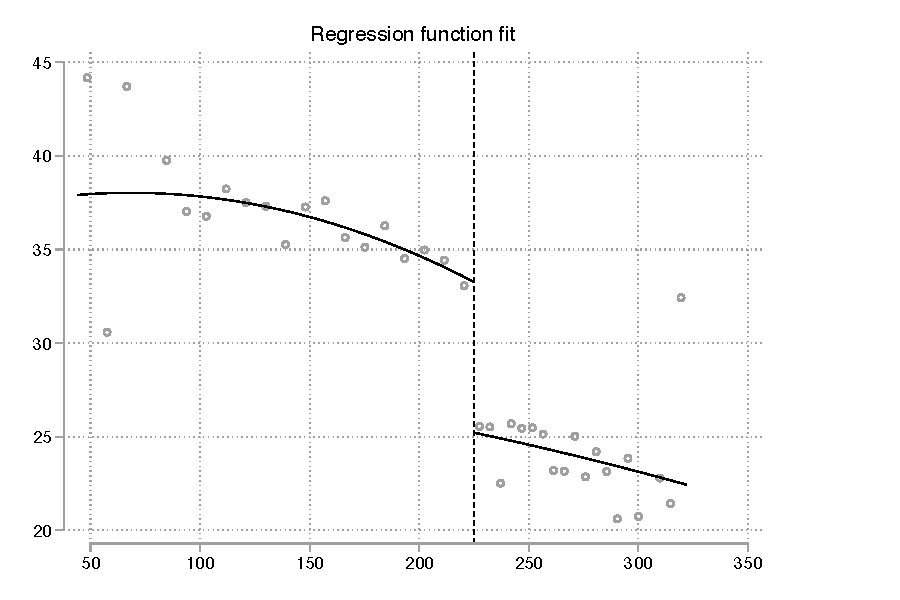
\includegraphics[scale = 0.7]{Q1b.pdf}
    \caption{A plot of the results using rdplot}
    \label{fig:Q1b}
\end{figure}
\bigskip
\noindent
\\ 2.
\\ To the best of my current understanding, I believe it is a valid instrument to some degree. 1) It causes variation in the treatment variable. With the strange policy, every vehicle equipped with the technology is significantly less fuel-efficient. 2) However, it might have a direct effect on the outcome variable $price$ through other mechanisms than $mpg$. For example, a longer/bigger vehicle tend to be safer and prettier and cost more materials to produce. The vehicle is therefore more expensive.  


\end{document}

